\section{Despliegue de información al usuario}

\subsection{Consultas}

Las consultas son desplegadas al usuario utilizando una librería conocida como \textit{DataTables}\footnote{Para mayor información consultar: \url{http://datatables.net/}, Noviembre 2012} que es un complemento para \textit{JQuery} que permite filtrar información y realizar búsquedas para facilitar su lectura.
\\\\
A continuación en la figura \ref{fig:consultaUsuario} se muestra un ejemplo de como se despliegua una consulta a un usuario.

\begin{figure}[H]
	\centering
	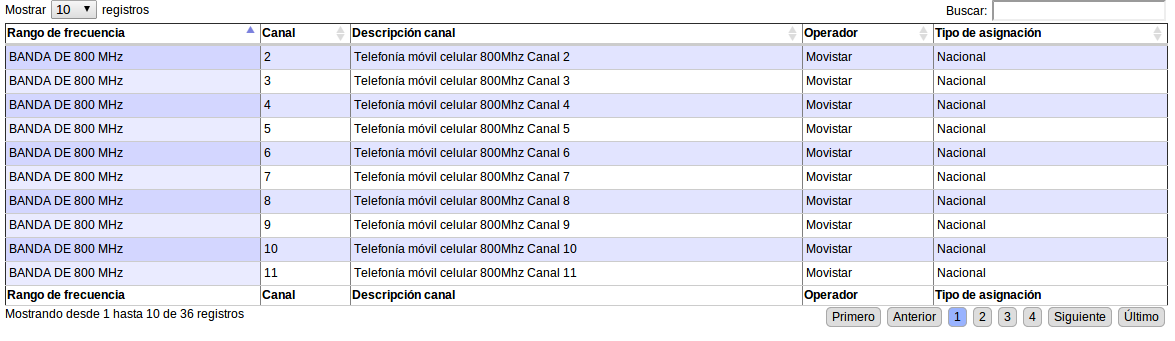
\includegraphics[width=15cm]{Capitulo8InterfacesWeb/Imagenes/ConsultaUsuario.png}
	\caption{Ejemplo de consulta a base de datos.}
	\label{fig:consultaUsuario}	
\end{figure}


\subsection{Archivos de entrada y salida}

El contenido de los archivos de entrada y salida pueden ser consultados en los módulos de Gestión de entradas y salidas respectivamente, a continuación en la figura \ref{fig:consultaEntrada} se muestra un despliegue de una entrada XML.

\begin{figure}[H]
	\centering
	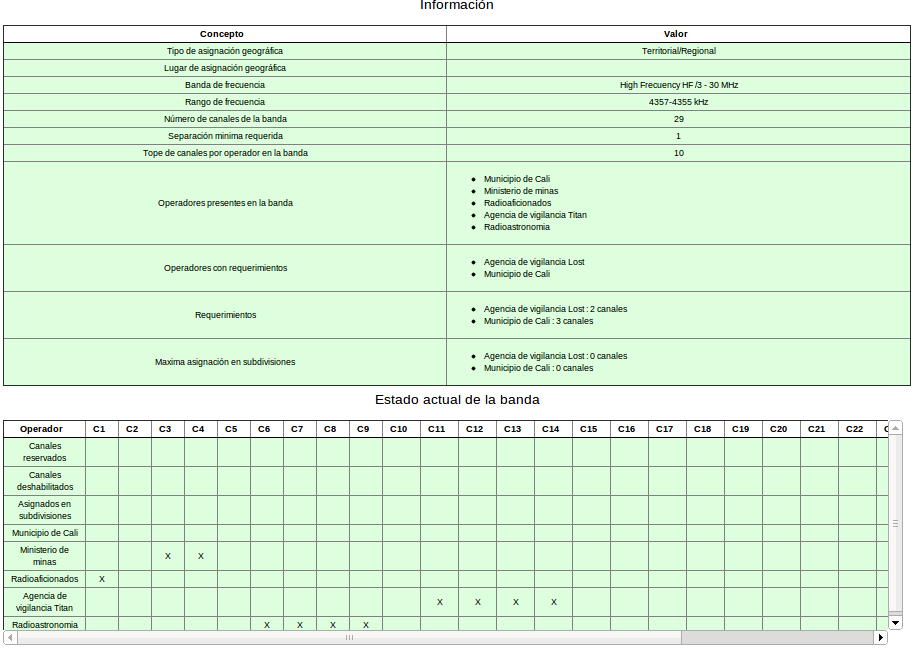
\includegraphics[width=14cm]{Capitulo8InterfacesWeb/Imagenes/Entrada.png}
	\caption{Despliegue información de la entrada.}
	\label{fig:consultaEntrada}	
\end{figure}

Para el caso de las salidas el despliegue es el mismo al de los resultados en los aplicativos, la diferencia es que se muestran todas las soluciones y no una en particular.

\subsection{Resultados}

Cada archivo de salida contiene una o más soluciones encontradas de una instancia del problema, estas contienen información acerca de los parámetros de ejecución y los costos de cada solución, en la figura \ref{fig:infoGeneral} se puede observar como se despliega el usuario la información general de la aplicación y en la figura \ref{fig:infoSolucion} se muestra la información en particular para una solución encontrada para una instancia.

\begin{figure}[H]
	\centering
	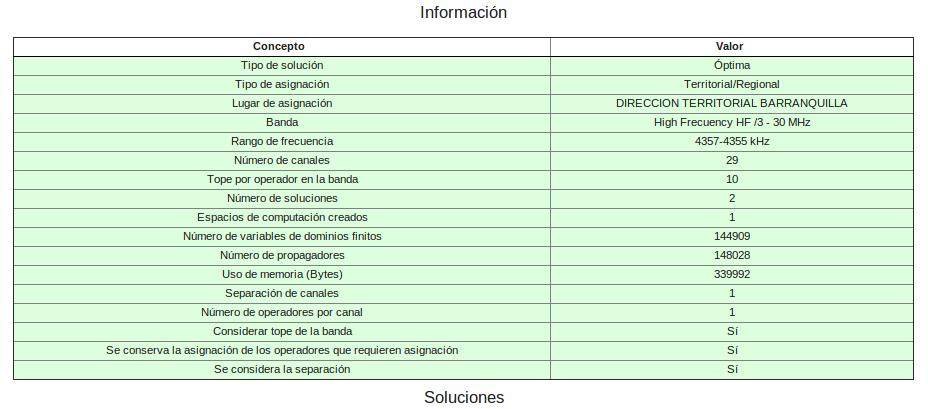
\includegraphics[width=15cm]{Capitulo8InterfacesWeb/Imagenes/InformacionGeneral.png}
	\caption{Ejemplo de consulta a base de datos.}
	\label{fig:infoGeneral}	
\end{figure}

\begin{figure}[H]
	\centering
	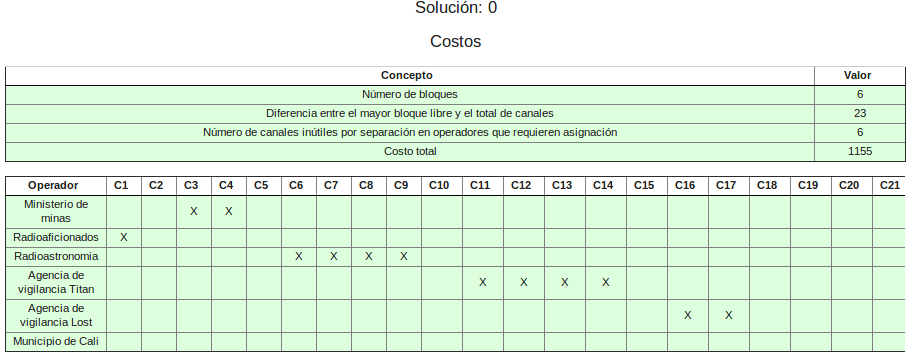
\includegraphics[width=15cm]{Capitulo8InterfacesWeb/Imagenes/Costos.png}
	\caption{Ejemplo de consulta a base de datos.}
	\label{fig:infoSolucion}	
\end{figure}



